\documentclass[11pt]{article}

\usepackage[T1]{fontenc}      % needed for \DJ (Đ in "Đoković")
\usepackage[margin=1in]{geometry}
\usepackage{amsmath,amssymb,amsthm,mathtools}
\usepackage{longtable}
\usepackage{graphicx}
\usepackage{hyperref}

\newtheorem{theorem}{Theorem}
\newtheorem{lemma}{Lemma}
\newtheorem{corollary}{Corollary}
\newtheorem{remark}{Remark}

\newcommand{\F}{\mathbb F}
\newcommand{\Z}{\mathbb Z}
\newcommand{\J}{J}
\newcommand{\I}{I}
\newcommand{\Rcal}{\mathcal R}

\title{A Paley--II analogue of the Scarpis--\DJ okovi\'c construction\\
       for prime powers \(q\equiv 1\pmod 4\)}
% Edit author/affiliation as appropriate before submission.
\author{Jeffery Kline}
\date{\today}

\begin{document}

\maketitle

\begin{abstract}
A Hadamard matrix of order \(m\) is a \(\{1,-1\}\)-matrix \(H\) with
\(HH^{T}=mI_{m}\).  Scarpis (1898) showed that for a prime
\(p\equiv 3\pmod 4\) a Hadamard matrix of order \(p+1\) can be lifted to
one of order \(p(p+1)\), and \DJ okovi\'c extended the lift to all prime
powers \(q\equiv 3\pmod 4\), asking for the analogous procedure for
\(q\equiv 1\pmod 4\).  That case was settled by Farouk and Wang (2020),
who lift an input Hadamard matrix of order \(2(q+1)\), subject to
eligibility conditions, to one of order \(2q(q+1)\), verifying
orthogonality by row-pair counting arguments in which the key inner
products are imported from the Hadamard property of the input matrix.
This note contributes a different method, not a new existence result.
Both routes are constructive; the difference is procedure versus
formula: their lift takes choices --- an input matrix and a bijection
--- that can change the output, while the matrix here is given by a
choice-free closed form, one matrix for each \(q\).  There is no input
matrix: the finite bands are given entrywise in
closed form by the quadratic character on \(\F_q\) composed with the
\(2\times 2\) Paley--II replacement blocks, and the Hadamard property
is proved by four block-Gram identities computed directly from
character sums.  The outputs differ as well: at \(q=5\) our matrix is
not Hadamard-equivalent to the order-\(60\) example printed by Farouk
and Wang.  We also make the family's coverage explicit:
every order \(2q(q+1)\) whose odd part is at most \(3000\) is already
recorded in the
standard tables, and the smallest order lying beyond that audited range,
\(q=81\) (order \(13284=4\cdot 41\cdot 81\)), also follows from a
classical Turyn product using \(T\)-matrices of order \(41\) and
Williamson-type matrices of order \(81=9^{2}\).  We exhibit the
witnessing constructions, identify the smallest
unaudited order, and
tabulate, for \(q\le3000\), those orders for which a deliberately
restricted elementary screen supplies no witness, emphasising that these
are \emph{unaudited} rather than open.
\end{abstract}

\section{Introduction}

For a prime power \(q\) let \(\F=\F_q\) and let
\(\chi\colon\F\to\{0,\pm1\}\) be the quadratic character,
\(\chi(0)=0\), \(\chi(x)=1\) for nonzero squares and \(-1\) otherwise.
Paley's two constructions split on the residue of \(q\): for
\(q\equiv 3\pmod 4\) Paley~I gives a Hadamard matrix of order \(q+1\),
and for \(q\equiv 1\pmod 4\) Paley~II gives one of order \(2(q+1)\)
\cite{Paley1933}.

Scarpis \cite{Scarpis1898} showed that for a prime \(p\equiv 3\pmod 4\) a
Hadamard matrix of order \(p+1\) lifts to one of order \(p(p+1)\).
\DJ okovi\'c \cite{Djokovic2016} replaced the prime by an arbitrary prime
power: if \(q\equiv 3\pmod 4\) is a prime power there is a Hadamard
matrix of order \(q(q+1)\); his note closes with the open problem of an
analogous procedure for \(q\equiv 1\pmod 4\).

Because the Paley--II seed has order \(2(q+1)\), the natural
Scarpis-type target in the \(q\equiv 1\pmod 4\) case is
\[
        q\cdot 2(q+1)=2q(q+1).
\]
We construct such a matrix directly from \(\chi\).  Throughout, \(q\equiv
1\pmod 4\) is a prime power, so \(\chi(-1)=1\); this is the only place
the residue class is used, and it is exactly what fails for
\(q\equiv 3\pmod 4\).

The existence of Hadamard matrices of order \(2q(q+1)\) for prime powers
\(q\equiv1\pmod4\) is due to Farouk and Wang \cite{FaroukWang2020}; the
contribution of this note is the method of
construction and proof.  Farouk and Wang obtain the matrix as the output
of a lifting procedure applied to an input Hadamard matrix of order
\(2(q+1)\) meeting certain eligibility conditions, and their verification
proceeds row pair by row pair, by counting arguments in which the key
inner-product values are imported from the Hadamard property of the
input matrix.  Here there is no input matrix: the finite bands are
written entrywise in the closed form \(\psi(\chi(y-x-t))\), and the
Hadamard property follows from four block-Gram identities whose
ingredients are computed directly from the quadratic character --- the
sums \eqref{eq:rowsum} and \(\sum_{z}\chi(z(z-d))=-1\), together with
the block identity \(P+ZR=0\).  The proof is thus self-contained at the
level of character sums, and the single place where the residue class
enters, \(\chi(-1)=1\), is isolated.  A secondary contribution is the
coverage analysis of Appendix~\ref{app:coverage}, which has no
counterpart in \cite{FaroukWang2020}: it locates the initial range
against audited tables of known Hadamard orders and applies a restricted
elementary screen beyond that range.

\section{The Paley--II blocks}

Put
\[
P=\begin{pmatrix}1&1\\ 1&-1\end{pmatrix},\quad
Z=\begin{pmatrix}1&-1\\ -1&-1\end{pmatrix},\quad
R=\begin{pmatrix}0&-1\\ 1&0\end{pmatrix},
\]
and let \(\psi\colon\{0,\pm1\}\to\{\pm1\}^{2\times2}\) be
\(\psi(0)=Z\), \(\psi(1)=P\), \(\psi(-1)=-P\); these are the Paley--II
replacement blocks, and \(ZR=-P\).  Write \(\Rcal=\J_q\otimes I_2\),
where \(\J_q\) is the \(q\times q\) all-ones matrix.  We use repeatedly
\[
        \sum_{u\in\F}\psi(\chi(u))=Z,
        \tag{2.1}\label{eq:rowsum}
\]
which holds because the nonzero squares and non-squares are equinumerous.

\section{The construction}

For \(t\in\F\) let \(K_t\) be the \(2q\times2q\) matrix with rows and
columns indexed by pairs \((x,a)\), \(x\in\F\), \(a\in\{0,1\}\), whose
\(2\times2\) block in position \((x,y)\) is
\[
        K_t[x,y]=\psi\bigl(\chi(y-x-t)\bigr).
\]

\begin{lemma}\label{lem:self}
For every \(t\in\F\), \(\;K_tK_t^{T}=2(q+1)I_{2q}-2\Rcal.\)
\end{lemma}

\begin{proof}
The \((x,x')\) block of \(K_tK_t^{T}\), with \(d=x'-x\) and
\(z=y-x-t\), equals \(\sum_{z}\psi(\chi(z))\psi(\chi(z-d))^{T}\).  For
\(d=0\) each summand is \(2I_2\), giving \(2qI_2\).  For \(d\neq0\) the
terms \(z=0\) and \(z=d\) carry opposite skew parts and cancel, using
\(\chi(-d)=\chi(d)\) (here \(\chi(-1)=1\)); for \(z\neq0,d\),
\(\psi(\chi(z))\psi(\chi(z-d))^{T}=2\chi(z)\chi(z-d)I_2\), and
\(\sum_z\chi(z(z-d))=-1\) yields \(-2I_2\).  These are the diagonal and
off-diagonal blocks of \(2(q+1)I-2\Rcal\).
\end{proof}

\begin{lemma}\label{lem:cross}
For \(r,s\in\F\),
\[
        \sum_{a\in\F}K_{ar}K_{as}^{T}=
        \begin{cases}
        2q(q+1)I_{2q}-2q\Rcal,&r=s,\\
        2\Rcal,&r\neq s.
        \end{cases}
\]
\end{lemma}

\begin{proof}
The case \(r=s\) is \(q\) copies of Lemma~\ref{lem:self}.  For
\(r\neq s\), in the \((x,x')\) block put \(z=y-x-ar\); the second
argument becomes \(z-(x'-x)+a(r-s)\), which ranges over all of \(\F\)
independently of \(z\) as \(a\) does.  By \eqref{eq:rowsum} each block is
\(Z Z^{T}=2I_2\), i.e.\ the corresponding block of \(2\Rcal\).
\end{proof}

For \(r\in\F\) let \(B_r\) be the \(2q\times2q\) matrix whose row
\((x,a)\) equals row \((r,a)\) of \(K_0\) for every \(x\); thus \(B_r\)
has only two distinct rows.  From Lemma~\ref{lem:self},
\(B_rB_s^{T}=2q\Rcal\) if \(r=s\) and \(-2\Rcal\) if \(r\neq s\).

Form the \(2q\times2q(q+1)\) block rows
\(M_r=\bigl[\,B_r\mid K_{ar}\ (a\in\F)\,\bigr].\)

\begin{lemma}\label{lem:finite}
\(M_rM_s^{T}=2q(q+1)I_{2q}\) if \(r=s\), and \(0\) if \(r\neq s\).
\end{lemma}

\begin{proof}
\(M_rM_s^{T}=B_rB_s^{T}+\sum_aK_{ar}K_{as}^{T}\).  For \(r=s\) the
\(2q\Rcal\) of the border cancels the \(-2q\Rcal\) of
Lemma~\ref{lem:cross}; for \(r\neq s\) the \(-2\Rcal\) cancels the
\(2\Rcal\).
\end{proof}

Let \(C\) be the Paley conference matrix indexed by
\(\{\infty\}\cup\F\), namely \(C_{u,u}=0\),
\(C_{\infty,x}=C_{x,\infty}=1\), \(C_{x,y}=\chi(y-x)\), and let \(S\) be
the order-\(2(q+1)\) Paley--II Hadamard matrix obtained by replacing
\(0,1,-1\) by \(Z,P,-P\).  Delete the two rows of \(S\) indexed by
\(\infty\); in each remaining row repeat the \(\infty\)-column pair
\(q\) times unchanged, and replace each finite column pair by its
product with \(R\), repeated \(q\) times.  This is a
\(2q\times2q(q+1)\) matrix \(M_\infty\).

\begin{lemma}\label{lem:cap}
\(M_\infty M_\infty^{T}=2q(q+1)I_{2q}\) and \(M_\infty M_r^{T}=0\) for all
\(r\in\F\).
\end{lemma}

\begin{proof}
The first identity holds because \(S\) is Hadamard, each column pair is
repeated \(q\) times, and right multiplication by \(R\) preserves row
inner products.  For the cross identity, summing a cap row against a row
of \(M_r\) and using \eqref{eq:rowsum} on every \(2q\)-block leaves
\(\bigl(P_\alpha+(\sum_{a}S[e,a]_\alpha)R\bigr)\cdot Z_\beta\); the inner
sum of finite entries of a row of \(S\) is \(Z_\alpha\), and
\(P+ZR=P-P=0\).
\end{proof}

\begin{theorem}\label{thm:main}
Let \(q\equiv1\pmod4\) be a prime power.  Then
\[
        H=\begin{bmatrix}M_\infty\\ M_r\ (r\in\F)\end{bmatrix}
\]
is a Hadamard matrix of order \(2q(q+1)\).
\end{theorem}

\begin{proof}
\(H\) is \(\{1,-1\}\) and square of order \(2q+q\cdot2q=2q(q+1)\).
Lemmas~\ref{lem:finite} and \ref{lem:cap} give
\(HH^{T}=2q(q+1)I\).
\end{proof}

\begin{corollary}
For every prime power \(q\equiv1\pmod4\) there is a Hadamard matrix of
order \(2q(q+1)\); the smallest non-prime instance is \(q=9\), of order
\(180\).
\end{corollary}

The construction has been verified by full Gram computation for all
\(q\le49\) (orders \(60,\dots,4900\), including the extension fields
\(q=9,25,49\)) and by streamed row-orthogonality checks for \(q=81\) and
\(q=125\) (orders \(13284\) and \(31500\)).

\section{Relation to the Farouk--Wang construction}

Theorem~\ref{thm:main} gives, for the \(q\equiv1\pmod4\) case, an
explicit form of the Scarpis-type family that \DJ okovi\'c
\cite{Djokovic2016} asked for.  That family was already constructed by
Farouk and Wang \cite{FaroukWang2020,FaroukWang2022} from the same
order-\(2(q+1)\) Paley--II seed.  This section records how the two
routes differ and where the orders of the family sit relative to the
audited tables of known Hadamard orders.

While Theorem~\ref{thm:main} and \cite[Cor.~2.1]{FaroukWang2020} assert
the same existence result, the routes differ.  Farouk and Wang obtain
the order-\(2q(q+1)\) matrix from a lifting procedure applied to a
Hadamard matrix of order \(2(q+1)\) satisfying the eligibility
conditions of \cite[Lem.~2.2]{FaroukWang2020} --- a formally larger
input class, with Paley~II the only exhibited member --- and verify
orthogonality row pair by row pair through counting arguments (row
sums, balanced sign-pair tallies, and a unique-intersection
computation), importing the key inner-product values from the Hadamard
property of the input matrix.  The present note fixes the Paley--II
seed and writes the finite bands entrywise in the closed form
\(\psi(\chi(y-x-t))\); the Hadamard property follows from four
block-Gram identities in which the corresponding quantities are
computed directly from the character sums \eqref{eq:rowsum} and
\(\sum_{z}\chi(z(z-d))=-1\), together with \(P+ZR=0\) and the
Hadamard property of the Paley--II seed \(S\) (itself a
character-sum identity).  The
correspondence is exact: their unique-intersection index matches the
affine collision \(x+ar=x'+as\) in the substitution step of
Lemma~\ref{lem:cross}, and their imported inner products match the
values that Lemma~\ref{lem:self} derives from
\(\sum_{z}\chi(z(z-d))=-1\).  The devices used for the cap band also
differ: a column permutation arranging balanced sign pairs in
\cite{FaroukWang2020} versus right multiplication by \(R\) here.  The
two constructions moreover produce genuinely different matrices, not
merely different presentations: at \(q=5\) the matrix of
Theorem~\ref{thm:main} is not Hadamard-equivalent to the order-\(60\)
example printed in the appendix of \cite{FaroukWang2020} --- the
multiset of absolute row-quadruple correlations
\(\bigl|\sum_{c}h_{ic}h_{jc}h_{kc}h_{lc}\bigr|\), an invariant of
Hadamard equivalence, differs for the two matrices
(Figure~\ref{fig:q5sbs}).  Since Farouk and
Wang note that their output may vary with the choice of bijection
\(\alpha\), we leave open whether the matrix of
Theorem~\ref{thm:main} is equivalent to some other output of their
procedure.

\begin{figure}[t]
\centering
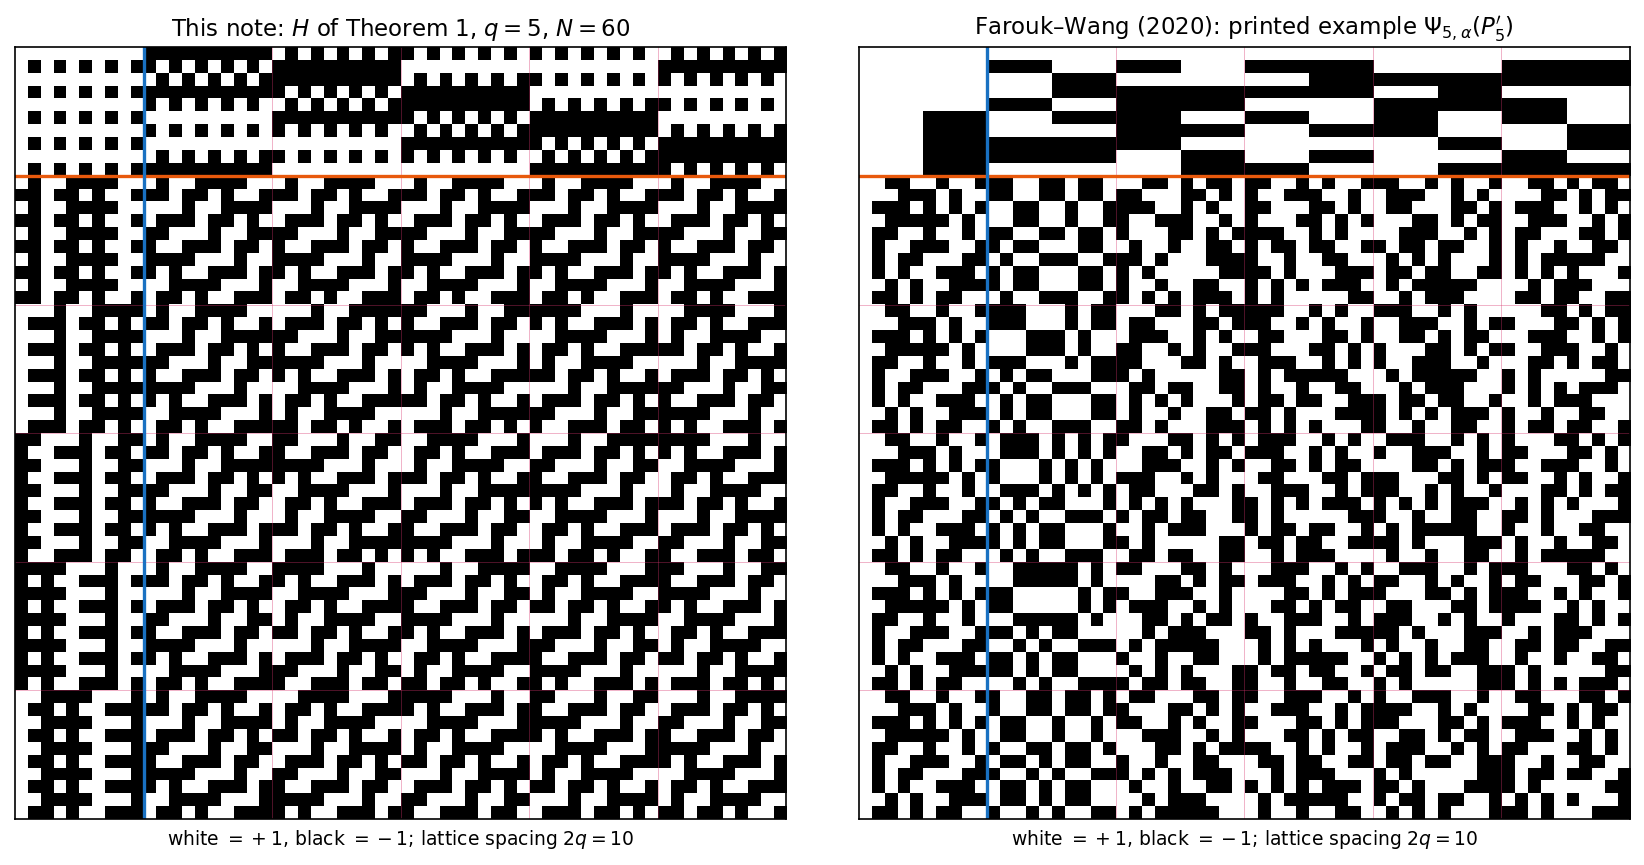
\includegraphics[width=\textwidth]{images/q5_side_by_side}
\caption{The two constructions at \(q=5\) (order \(60\); white
\(=+1\), black \(=-1\); lattice spacing \(2q=10\)).  Left: the matrix
of Theorem~\ref{thm:main} --- the cap band \(M_\infty\) above the
orange separator is a family of period-two column patterns, and the
finite bands \(M_r\) carry the diagonal texture of the shifts
\(\psi(\chi(y-x-ar))\).  Right: the order-\(60\) example
\(\Psi_{5,\alpha}(P_5')\) printed in the appendix of
\cite{FaroukWang2020}, whose top band is a coarse tiling (its border
block consists of four constant \(5\times5\) quadrants) and whose
finite bands show no diagonal structure.  The two matrices are
Hadamard-inequivalent: over the \(\binom{60}{4}=487{,}635\) row
quadruples, the right matrix attains
\(\bigl|\sum_{c}h_{ic}h_{jc}h_{kc}h_{lc}\bigr|=28\) on \(400\)
quadruples, the left on none, and this multiset is invariant under row
and column permutations and negations (and the comparison fails in
both orientations, covering the transpose convention as well).  This
separates the printed representative only: outputs of the Farouk--Wang
procedure for other choices of \(\alpha\) are not addressed.}
\label{fig:q5sbs}
\end{figure}

Since \(q\equiv1\pmod4\), the \(2\)-adic valuation of the order is
exactly \(2\):
\[
        2q(q+1)=4\cdot q\cdot\tfrac{q+1}{2},
        \qquad q\ \text{and}\ \tfrac{q+1}{2}\ \text{both odd.}
        \tag{4.1}\label{eq:fourodd}
\]
Thus every order is \(4\times(\text{odd})\), so it is never a Kronecker
product of two smaller Hadamard matrices, and its odd part
\(q(q+1)/2\) is always composite.  Two consequences follow.  First, the
family never meets the dominant list of open Hadamard orders, which are
\(4\times\text{prime}\).  Second, \eqref{eq:fourodd} has the form needed
for Turyn's construction: when \(T\)-matrices of order \(t\) and
Williamson-type matrices of order \(w\) are available, one obtains a
Hadamard matrix of order \(4tw\)
\cite{Turyn1974,SeberryYamada1992}, and here \(\{t,w\}=\{q,(q+1)/2\}\).
The coverage analysis of Appendix~\ref{app:coverage} makes both points
quantitative: all orders with odd part \(\le 3000\) are recorded in the
standard tables, the first order beyond that range is covered by such a
Turyn product, and a restricted screen beyond the audited range records
exactly which orders it does and does not cover.  Failure of that screen is
not a claim that an order is open.

\appendix

\section{Coverage analysis}\label{app:coverage}

Write \(N=2q(q+1)\) and \(m=q(q+1)/2\) for its odd part, so
\(N=4m\).  We assess coverage of \(N\) by prior constructions on three
levels: the audited tables (\S\ref{app:audit}), the first unaudited
order (\S\ref{app:81}), and an elementary-witness test that isolates
candidate orders (\S\ref{app:candidates}).

\subsection{Orders with odd part at most \texorpdfstring{\(3000\)}{3000}}
\label{app:audit}

The surveys of Seberry and Yamada \cite{SeberryYamada1992,
SeberryYamada2020} and the database of Cati and Pasechnik
\cite{CatiPasechnik2024} record, for every odd \(m\le 3000\), the least
\(t\) for which a Hadamard matrix of order \(2^{t}m\) is known.  The
default is \(t=2\) (so \(N=4m\) is known), and the only odd \(m\le3000\)
with \(t>2\) are the primes \(167,179,223,283\) (orders \(668,716,892,1132\),
still open).  Since \(m=q(q+1)/2\) is composite it is never one of these;
hence \emph{every \(N\) with \(m\le3000\) is a known Hadamard order}.
This is the range \(q\le73\), tabulated below with an explicit
elementary witness where one exists (Paley~I/II, or a Turyn product
\(4tw\)).

\begin{center}
\begin{tabular}{r r l l}
\(q\) & \(N=2q(q+1)\) & odd part \(m\) & witnessing construction\\\hline
5  & 60    & \(3\cdot5\)        & Paley II, \(p=29\)\\
9  & 180   & \(3^{2}\cdot5\)    & Paley II, \(p=89\)\\
13 & 364   & \(7\cdot13\)       & Paley II, \(p=181\)\\
17 & 612   & \(3^{2}\cdot17\)   & Turyn \(4\cdot9\cdot17\)\\
25 & 1300  & \(5^{2}\cdot13\)   & Turyn \(4\cdot13\cdot25\)\\
29 & 1740  & \(3\cdot5\cdot29\) & Turyn \(4\cdot15\cdot29\)\\
37 & 2812  & \(19\cdot37\)      & Turyn \(4\cdot19\cdot37\)\\
41 & 3444  & \(3\cdot7\cdot41\) & Paley II, \(p=1721\)\\
49 & 4900  & \(5^{2}\cdot7^{2}\)& Turyn \(4\cdot25\cdot49\)\\
53 & 5724  & \(3^{3}\cdot53\)   & Paley II, \(p=2861\)\\
61 & 7564  & \(31\cdot61\)      & Turyn \(4\cdot31\cdot61\)\\
73 & 10804 & \(37\cdot73\)      & tables; no restricted witness (see \S\ref{app:candidates})\\
\end{tabular}
\end{center}

\noindent
The entry \(q=73\) is instructive: the restricted test below supplies no
divisor-split witness for its odd part \(2701=37\cdot73\), yet
\(N=10804\) is a known Hadamard order because \(m\le3000\) is audited.
Failure of the elementary test is therefore a property of that test, not
of Hadamard existence.

\subsection{The first unaudited order: \texorpdfstring{\(q=81\)}{q=81}}
\label{app:81}

The smallest order of the family whose odd part exceeds \(3000\), and
hence lies beyond the audited range, is
\[
        q=81=3^{4},\qquad N=13284,\qquad m=3321=3^{4}\cdot41>3000 .
\]
It is nevertheless a known Hadamard order.  By \eqref{eq:fourodd},
\[
        13284 = 4\cdot 41\cdot 81 = 4tw,\qquad t=41,\ w=81,
\]
and both ingredients are classical: \(T\)-matrices of order \(41\) come
from the base sequences \(BS(21,20)\) \cite{Turyn1974,
KharaghaniTayfehRezaie2005}, and Williamson-type matrices of order
\(81=9^{2}\) come from Turyn's \(9\)-power family
\cite{Turyn1974,SeberryYamada1992}.  The Turyn array on these
\cite{SeberryYamada1992,SeberryYamada2020} yields a Hadamard matrix of
order \(4\cdot41\cdot81=13284\).  Thus \(q=81\) is the smallest unaudited
order, and it is covered.

\subsection{An elementary-witness test and the candidate orders}
\label{app:candidates}

Beyond the audited range we have no table to appeal to, so we apply a
deliberately conservative \emph{elementary-witness} test based on
\eqref{eq:fourodd} and Turyn's array.  We call an odd order \(t\)
\emph{\(T\)-known} when \(t\le59\); the required \(T\)-matrices follow
from the known base sequences
\(BS((t+1)/2,(t-1)/2)\), whose second parameter is at most \(29\).
We call an odd order \(w\) \emph{\(W\)-known} when \(w\le33\), or when
\(2w-1\) is a prime power; in the latter case Turyn's
\((P+1)/2\) family, with \(P=2w-1\equiv1\pmod4\), supplies the required
Williamson-type matrices.  An unaudited order \(N=4m\) passes the test
if \(N\) is a Paley~I/II order, or if there is an \emph{exhibited}
factorization
\[
        m=tw,\qquad t\ \hbox{\(T\)-known},\qquad
        w\ \hbox{\(W\)-known}.
        \tag{C.1}\label{eq:strictwitness}
\]
Thus every passing verdict is an unconditional construction from the
ingredients just listed; no multiplicative closure is assumed.

\begin{remark}\label{rem:mult}
An earlier version of this appendix asserted that classes of eligible
\(T\)- and Williamson orders were multiplicatively closed and then
classified \(m\) prime factor by prime factor.  That assertion was uncited,
and we withdraw both it and the factorwise test.  Even for Williamson
matrices proper, unrestricted closure is false:
\DJ okovi\'c \cite{Djokovic1993} enumerated Williamson matrices at orders
\(33\) and \(39\), but proved that none exist at
\(35=5\cdot7\), although they exist at both orders \(5\) and \(7\).
Holzmann, Kharaghani and Tayfeh-Rezaie
\cite{HolzmannKharaghaniTayfehRezaie2008} later found the further
nonexistence orders \(47\), \(53\), and \(59\).  Terminology in the
literature includes broader variants called Williamson-type matrices;
we make no closure claim for any such class.  Instead,
\eqref{eq:strictwitness} requires the two actual ingredient orders used
by Turyn's array to be known individually.

The factorwise test was unreliable in both directions.  It could accept
an \(m\) merely because each prime factor was eligible, without producing
a pair \(t,w\).  It could also reject an \(m\) because of a prime factor
that nevertheless lies inside a directly known composite \(W\)-order.
For example, at \(q=197\),
\[
        m=19503=3\cdot6501,\qquad 2\cdot6501-1=13001
\]
is prime, so \(t=3,w=6501\) is a witness under
\eqref{eq:strictwitness}; the old factorwise test rejected it because of
the prime factor \(197\).  This is why the table below is recomputed from
actual divisor splits rather than inherited from the earlier screen.

The audited range of \S\ref{app:audit} is a table lookup, and the
\(q=81\) witness of \S\ref{app:81} cites its two ingredients
individually.  Both are independent of this correction.  Nothing in
\S\S1--4, and in particular neither Theorem~\ref{thm:main} nor its proof,
depends on this appendix.
\end{remark}

A passing verdict now exhibits a construction.  A failing verdict
(\emph{no restricted elementary witness}) is a statement about this test
only, not a claim that \(N\) is open.  Over the \(232\) orders with
\(q\le3000\), the strict test covers \(128\) (audited, Paley, or Turyn)
and leaves \(104\) without a witness.  The smallest failure remains
\[
        q=109,\qquad N=23980,\qquad m=5\cdot11\cdot109,
\]
for which none of the possible \(T\)-known divisors produces a
\(W\)-known complementary factor.  In particular,
\(2\cdot109-1=217=7\cdot31\) is not a prime power.  This
\(N=23980\) is the smallest order of the family for which we exhibit
neither an audited entry nor a restricted elementary witness; we do not
assert it is open.  Williamson-type matrices of order \(109\), if
available, would settle it at once using \(t=55,w=109\) (compare
\(q=73\)).

Table~\ref{tab:candidates} lists all \(104\) failures of this restricted
test for \(q\le3000\).  It is a reproducible classification relative to
the stated ingredient sets, not a literature-complete classification of
the corresponding Hadamard orders.

{\footnotesize
\begin{longtable}{r r l}
\caption{Orders \(N=2q(q+1)\), \(q\) a prime power \(\equiv1\pmod4\),
with no restricted elementary witness (\S\ref{app:candidates}),
\(109\le q\le2969\).}\label{tab:candidates}\\
\hline
\(q\) & \(N\) & odd part \(m\)\\\hline
\endfirsthead
\hline
\(q\) & \(N\) & odd part \(m\)\\\hline
\endhead
\hline
\endfoot
109 & 23980 & \(5\cdot11\cdot109\) \\
121 & 29524 & \(11^{2}\cdot61\) \\
157 & 49612 & \(79\cdot157\) \\
173 & 60204 & \(3\cdot29\cdot173\) \\
229 & 105340 & \(5\cdot23\cdot229\) \\
277 & 154012 & \(139\cdot277\) \\
289 & 167620 & \(5\cdot17^{2}\cdot29\) \\
313 & 196564 & \(157\cdot313\) \\
397 & 316012 & \(199\cdot397\) \\
409 & 335380 & \(5\cdot41\cdot409\) \\
421 & 355324 & \(211\cdot421\) \\
457 & 418612 & \(229\cdot457\) \\
529 & 560740 & \(5\cdot23^{2}\cdot53\) \\
577 & 667012 & \(17^{2}\cdot577\) \\
601 & 723604 & \(7\cdot43\cdot601\) \\
613 & 752764 & \(307\cdot613\) \\
617 & 762612 & \(3\cdot103\cdot617\) \\
641 & 823044 & \(3\cdot107\cdot641\) \\
661 & 875164 & \(331\cdot661\) \\
733 & 1076044 & \(367\cdot733\) \\
757 & 1147612 & \(379\cdot757\) \\
797 & 1272012 & \(3\cdot7\cdot19\cdot797\) \\
821 & 1349724 & \(3\cdot137\cdot821\) \\
829 & 1376140 & \(5\cdot83\cdot829\) \\
841 & 1416244 & \(29^{2}\cdot421\) \\
853 & 1456924 & \(7\cdot61\cdot853\) \\
877 & 1540012 & \(439\cdot877\) \\
937 & 1757812 & \(7\cdot67\cdot937\) \\
961 & 1848964 & \(13\cdot31^{2}\cdot37\) \\
997 & 1990012 & \(499\cdot997\) \\
1009 & 2038180 & \(5\cdot101\cdot1009\) \\
1021 & 2086924 & \(7\cdot73\cdot1021\) \\
1033 & 2136244 & \(11\cdot47\cdot1033\) \\
1097 & 2409012 & \(3^{2}\cdot61\cdot1097\) \\
1109 & 2461980 & \(3\cdot5\cdot37\cdot1109\) \\
1117 & 2497612 & \(13\cdot43\cdot1117\) \\
1129 & 2551540 & \(5\cdot113\cdot1129\) \\
1153 & 2661124 & \(577\cdot1153\) \\
1181 & 2791884 & \(3\cdot197\cdot1181\) \\
1201 & 2887204 & \(601\cdot1201\) \\
1213 & 2945164 & \(607\cdot1213\) \\
1237 & 3062812 & \(619\cdot1237\) \\
1249 & 3122500 & \(5^{4}\cdot1249\) \\
1297 & 3367012 & \(11\cdot59\cdot1297\) \\
1321 & 3492724 & \(661\cdot1321\) \\
1361 & 3707364 & \(3\cdot227\cdot1361\) \\
1373 & 3773004 & \(3\cdot229\cdot1373\) \\
1381 & 3817084 & \(691\cdot1381\) \\
1453 & 4225324 & \(727\cdot1453\) \\
1481 & 4389684 & \(3\cdot13\cdot19\cdot1481\) \\
1553 & 4826724 & \(3\cdot7\cdot37\cdot1553\) \\
1597 & 5104012 & \(17\cdot47\cdot1597\) \\
1601 & 5129604 & \(3^{2}\cdot89\cdot1601\) \\
1609 & 5180980 & \(5\cdot7\cdot23\cdot1609\) \\
1637 & 5362812 & \(3^{2}\cdot7\cdot13\cdot1637\) \\
1657 & 5494612 & \(829\cdot1657\) \\
1681 & 5654884 & \(29^{2}\cdot41^{2}\) \\
1709 & 5844780 & \(3^{2}\cdot5\cdot19\cdot1709\) \\
1753 & 6149524 & \(877\cdot1753\) \\
1777 & 6319012 & \(7\cdot127\cdot1777\) \\
1789 & 6404620 & \(5\cdot179\cdot1789\) \\
1873 & 7020004 & \(937\cdot1873\) \\
1877 & 7050012 & \(3\cdot313\cdot1877\) \\
1933 & 7476844 & \(967\cdot1933\) \\
2017 & 8140612 & \(1009\cdot2017\) \\
2029 & 8237740 & \(5\cdot7\cdot29\cdot2029\) \\
2053 & 8433724 & \(13\cdot79\cdot2053\) \\
2089 & 8732020 & \(5\cdot11\cdot19\cdot2089\) \\
2113 & 8933764 & \(7\cdot151\cdot2113\) \\
2137 & 9137812 & \(1069\cdot2137\) \\
2161 & 9344164 & \(23\cdot47\cdot2161\) \\
2197 & 9658012 & \(7\cdot13^{3}\cdot157\) \\
2209 & 9763780 & \(5\cdot13\cdot17\cdot47^{2}\) \\
2213 & 9799164 & \(3^{3}\cdot41\cdot2213\) \\
2269 & 10301260 & \(5\cdot227\cdot2269\) \\
2273 & 10337604 & \(3\cdot379\cdot2273\) \\
2281 & 10410484 & \(7\cdot163\cdot2281\) \\
2297 & 10557012 & \(3\cdot383\cdot2297\) \\
2341 & 10965244 & \(1171\cdot2341\) \\
2377 & 11305012 & \(29\cdot41\cdot2377\) \\
2381 & 11343084 & \(3\cdot397\cdot2381\) \\
2389 & 11419420 & \(5\cdot239\cdot2389\) \\
2401 & 11534404 & \(7^{4}\cdot1201\) \\
2417 & 11688612 & \(3\cdot13\cdot31\cdot2417\) \\
2437 & 11882812 & \(23\cdot53\cdot2437\) \\
2473 & 12236404 & \(1237\cdot2473\) \\
2557 & 13081612 & \(1279\cdot2557\) \\
2617 & 13702612 & \(7\cdot11\cdot17\cdot2617\) \\
2621 & 13744524 & \(3\cdot19\cdot23\cdot2621\) \\
2657 & 14124612 & \(3\cdot443\cdot2657\) \\
2689 & 14466820 & \(5\cdot269\cdot2689\) \\
2693 & 14509884 & \(3\cdot449\cdot2693\) \\
2713 & 14726164 & \(23\cdot59\cdot2713\) \\
2749 & 15119500 & \(5^{3}\cdot11\cdot2749\) \\
2777 & 15429012 & \(3\cdot463\cdot2777\) \\
2797 & 15652012 & \(1399\cdot2797\) \\
2801 & 15696804 & \(3\cdot467\cdot2801\) \\
2833 & 16057444 & \(13\cdot109\cdot2833\) \\
2837 & 16102812 & \(3\cdot11\cdot43\cdot2837\) \\
2857 & 16330612 & \(1429\cdot2857\) \\
2909 & 16930380 & \(3\cdot5\cdot97\cdot2909\) \\
2917 & 17023612 & \(1459\cdot2917\) \\
2953 & 17446324 & \(7\cdot211\cdot2953\) \\
2969 & 17635860 & \(3^{3}\cdot5\cdot11\cdot2969\) \\
\end{longtable}
}

\noindent
Every odd part in Table~\ref{tab:candidates} is composite by
\eqref{eq:fourodd}, so these orders do not meet the
\(4\times\text{prime}\) form that dominates the initial list of open
Hadamard orders.  At the larger sizes in the table we make no
literature-complete assertion of known or open status.  Widening the
ingredient set (for example with computer-tabulated Williamson and
\(T\)-matrices or Goethals--Seidel cyclotomic difference sets) can remove
entries from this restricted list.  The role of
Theorem~\ref{thm:main} is to give a single closed-form rule for the whole
family, including the region this elementary screen does not reach,
rather than to derive novelty from a coverage-table gap.

\begin{thebibliography}{99}

\bibitem{FaroukWang2020}
A.~Farouk and Q.-W.~Wang,
\newblock An infinite family of Hadamard matrices constructed from
  Paley type matrices,
\newblock {\em Filomat} 34 (2020), no.\ 3, 815--834.

\bibitem{FaroukWang2022}
A.~Farouk and Q.-W.~Wang,
\newblock Construction of new Hadamard matrices using known Hadamard
  matrices,
\newblock {\em Filomat} 36 (2022), no.\ 6, 2025--2042.

\bibitem{Hadamard1893}
J.~Hadamard,
\newblock R\'esolution d'une question relative aux d\'eterminants,
\newblock {\em Bull.\ Sci.\ Math.} 17 (1893), 240--246.

\bibitem{Paley1933}
R.~E.~A.~C.~Paley,
\newblock On orthogonal matrices,
\newblock {\em J.\ Math.\ Phys.} 12 (1933), 311--320.

\bibitem{Scarpis1898}
U.~Scarpis,
\newblock Sui determinanti di valore massimo,
\newblock {\em Rend.\ R.\ Ist.\ Lombardo Sci.\ Lett.} (2) 31 (1898),
  1441--1446.

\bibitem{Williamson1944}
J.~Williamson,
\newblock Hadamard's determinant theorem and the sum of four squares,
\newblock {\em Duke Math.\ J.} 11 (1944), 65--81.

\bibitem{Turyn1974}
R.~J.~Turyn,
\newblock Hadamard matrices, Baumert--Hall units, four-symbol sequences,
  pulse compression, and surface wave encodings,
\newblock {\em J.\ Combin.\ Theory Ser.\ A} 16 (1974), 313--333.

\bibitem{SeberryYamada1992}
J.~Seberry and M.~Yamada,
\newblock Hadamard matrices, sequences, and block designs,
\newblock in {\em Contemporary Design Theory} (J.~H.~Dinitz and
  D.~R.~Stinson, eds.), Wiley, 1992, pp.\ 431--560.

\bibitem{Djokovic1993}
D.~Z.~\DJ okovi\'c,
\newblock Williamson matrices of order \(4n\) for \(n=33,35,39\),
\newblock {\em Discrete Math.} 115 (1993), 267--271.
\newblock \url{https://doi.org/10.1016/0012-365X(93)90495-F}.

\bibitem{HolzmannKharaghaniTayfehRezaie2008}
W.~H.~Holzmann, H.~Kharaghani, and B.~Tayfeh-Rezaie,
\newblock Williamson matrices up to order 59,
\newblock {\em Des.\ Codes Cryptogr.} 46 (2008), no.\ 3, 343--352.
\newblock \url{https://doi.org/10.1007/s10623-007-9163-5}.

\bibitem{Djokovic2016}
D.~Z.~\DJ okovi\'c,
\newblock Generalization of Scarpis's theorem on Hadamard matrices,
\newblock arXiv:1601.00635, 2016.
\newblock \url{https://arxiv.org/abs/1601.00635}.

\bibitem{KharaghaniTayfehRezaie2005}
H.~Kharaghani and B.~Tayfeh-Rezaie,
\newblock A Hadamard matrix of order 428,
\newblock {\em J.\ Combin.\ Des.} 13 (2005), 435--440.
\newblock \url{https://doi.org/10.1002/jcd.20043}.

\bibitem{SeberryYamada2020}
J.~Seberry and M.~Yamada,
\newblock {\em Hadamard Matrices: Constructions using Number Theory and
  Linear Algebra},
\newblock Wiley, 2020.
\newblock \url{https://doi.org/10.1002/9781119520252}.

\bibitem{CatiPasechnik2024}
M.~Cati and D.~V.~Pasechnik,
\newblock A database of constructions of Hadamard matrices,
\newblock arXiv:2411.18897v2, 2025.
\newblock \url{https://arxiv.org/abs/2411.18897}.
\newblock \url{https://doi.org/10.48550/arXiv.2411.18897}.

\end{thebibliography}

\end{document}
